Consider the problem of optimizing an arbitrary continuous function $f: 𝓧 → ℝ$
where $𝓧 ⊂ ℝ^d, d ∈ ℕ$. We call $f$ the \emph{objective function} and treat it
as a black box, making no other assumptions on its analytical form, or on our
ability to compute its derivatives. Our goal is to find the global minimum
$\vx_\text{opt}$ over the set $𝓧$, that is
$$
\vx_\text{opt} = \arg\min_{\vx ∈ 𝓧} f(\vx).
$$

We also assume that the evaluation of $f$ is expensive, as the goal of bayesian
optimization is to find the optimum in as few evaluations as possible. Consider
the case when evaluating $f$ means performing a computation that is not only
time consuming, but for example also costs a lot of money. We might only have a
fixed budget which puts a hard limit on the number of evaluations we can
perform. If the function can be evaluated cheaply, other global optimization
approaches such as simulated annealing or evolution strategies could
potentially yield better results \ref{eva}.

Bayesian optimization techniques are some of the most efficient approaches in
terms of the number of function evaluations required. Much of the efficiency
stems from the ability to incorporate prior belief about the problem and to
trade of exploration and exploitation of the search space \citep{nando-bopt-tutorial}

It is called bayesian because it combines the prior knowledge $p(f)$ about the
function together with the data in the form of the likelihood $p(x|f)$ to
formulate a posterior distribution on the set of possible functions $p(f|x)$.
We will use the posterior distribution to figure out which point should be
evaluated next to give a likely improvement over the currently obtained
maximum. This improvement is defined by an \newterm{acquisition function},
\todo{mezera pred carkou} which represents our optimization objective. A simple
example of an acquisition function is the \newterm{probability of improvement},
which simply represents the probability of improving our objective compared to
the previously achieved maximum. We will show a few other examples of
acquisition functions in a later section \ref{section-acq-fn}.

The optimization procedure is sequential, using a bayesian posterior update at
each step, refining its model as more data are available. At each step the we
maximize the acquisition function in order to obtain the next sample point
$x_{i+1}$. We then evaluate $f(x_{i+1})$ to obtain $y_{i+1}$, and incorporate
it into the dataset. This processs is repeated for as many evaluations as we
can perform. See algorithm \ref{alg:bopt} for pseudocode.

\begin{algorithm}
  \label{alg:bopt}
  \DontPrintSemicolon
  \SetAlgoLined
  Initialize $\rx_1$ randomly and evaluate $y_1 = f(\rx_1), 𝓓_1 = {(\rx_1, y_1)}$. \;
  \For{$i = 1, 2, \ldots$}{
    Find $x_{i+1}$ by maximizing the acquisition function. \;
    Evaluate $y_{i+1} = f(\rx(x_{i+1})$. \;
    Add the sample to the dataset $𝓓_{i+1} = 𝓓_i \cup (\rx_{i+1}, y_{i+1})$. \;
    Update the Gaussian Process. \;
  }
  \caption{Bayesian Optimization, \cite{nando-bopt-tutorial}}
\end{algorithm}


At its core, bayesian optimization only requires two things. A probabilistic
regression model which combines prior beliefs $p(f)$ with the data. And an
acquistion function which describes the optimality of the next sampling point.

\section{Prior Distribution over Functions}

Bayesian methods by definition require a prior distribution over the quantity
of interest. Since we are building a probabilistic model over functions, we
need to obtain a prior distribution over functions, which will capture our
general beliefs about the properties of the objective function. For example, if
we knew that our function was periodic, we would want a prior distribution over
periodic functions. But in the case of hyperparameter optimization we will
generally only consider continuous functions.

We will follow the general consensus of using a Gaussian process (GP)
\todo{zkratkovat od zacatku} as a prior distribution over functions
\citep{nando-bopt-tutorial}, as it provides many nice theoretical properties, as well as
tractable posterior inference. A GP is an extension of the multivariate
Gaussian distribution to infinitely dimensional random variables. Just as a
multivariate Gaussian can be thought of as a distribution over vectors, a GP
can be thought of as a distribution over infinitely dimensional vectors, which
when indexed by the real numbers are equivalent to functions. A GP assumes that
any finite subset $\rx = (x_1, \ldots, x_n)$ is jointly Gaussian with some mean
$m(\rx)$ and covariance $Σ(\rx)$. A GP is defined by its mean function $m$ and
covariance function $k$ \citep{murphy2012machine}. We write
$$
  𝓖𝓟(m(\rx), k(\rx, \rx')).
$$

\begin{center}
  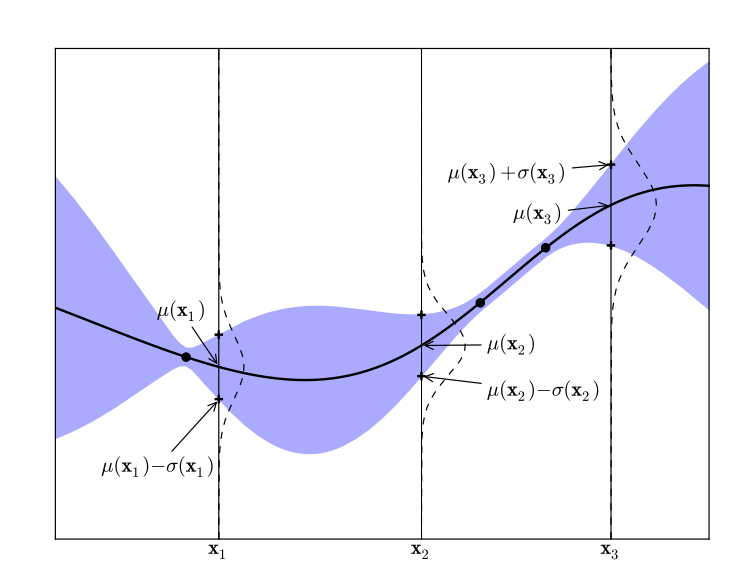
\includegraphics[width=0.8\textwidth]{images/gp-1d.png}
  \todo{ukradeny obrazek, referencovat nekde}
\end{center}

By convention, we assume that the prior mean is a constant zero function, that
is $m(x) = 0$. Since the data is often normalized in practice, this does not
reduce the flexibility of the model. The power of a GP comes from its
covariance function, which for any two points $\rx_i$ and $\rx_j$ defines their
covariance $k(\rx_i, \rx_j)$. If $\rx_i$ and $\rx_j$ have a high covariance,
the values of the function at those points will be similar.

Intuitively, it is often useful to think of a GP as a function, which instead
of returning a scalar $f(x)$ returns the mean and standard deviation of a
Gaussian distribution over the possible values, centered at $x$. We leave a formal
treatment of GPs until chapter~\ref{chapter:gp}.

---


% Bayesian optimization does not require any particular form of the prior
% distribution $p(f)$. We only need to have the ability to optimize the
% acquisition function to find the next sampling point $x$. In order to compute
% the acquisition function, we also need to have the ability to compute the
% posterior distribution $p(f|x)$. And as is the case with any other bayesian method,
%
%
% The prior distribution $p(f)$ allows the model to estimate
% the behavior of the function when data is lacking, but when more data becomes
% available, the likelihood overwhelms the prior during the posterior update
%
% Bayesian optimization is a sequential model-based approach to 
%
%
% In order to compute the posterior distribution $p(f|x)$ over functions, we need





\section{Acquisition Functions}

\section{Related work}
\section{Hyperparam vs. Architecture Search}
\section{Diskretni hyperparam vs onehot vs ...}

